% ========================================
% Header einbinden
% ========================================

\documentclass[bibtotoc,titlepage]{scrartcl}

% Deutsche Spracheinstellungen
\usepackage[ngerman,german]{babel, varioref}
\usepackage[T1]{fontenc}
\usepackage[utf8]{inputenc}

%\usepackage{marvosym}

\usepackage{amsfonts}
\usepackage{amssymb}
\usepackage{amsmath}
\usepackage{amscd}
\usepackage{amstext}

\usepackage{longtable}

%\usepackage{bibgerm}

\usepackage{footnpag}

\usepackage{ifthen}                 %%% package for conditionals in TeX
\usepackage[amssymb]{SIunits}
%Für textumflossene Bilder und Tablellen
%\usepackage{floatflt} - veraltet

%Für Testzwecke aktivieren, zeigt labels und refs im Text an.
%\usepackage{showkeys}

% Abstand zwischen zwei Absätzen nach DIN (1,5 Zeilen)
% \setlength{\parskip}{1.5ex plus0.5ex minus0.5ex}

% Einrückung am Anfang eines neuen Absatzes nach DIN (keine)
%\setlength{\parindent}{0pt}

% Ränder definieren
% \setlength{\oddsidemargin}{0.3cm}
% \setlength{\textwidth}{15.6cm}

% bessere Bildunterschriften
%\usepackage[center]{caption2}


% Problemlösungen beim Umgang mit Gleitumgebungen
\usepackage{float}

% Nummeriert bis zur Strukturstufe 3 (also <section>, <subsection> und <subsubsection>)
%\setcounter{secnumdepth}{3}

% Führt das Inhaltsverzeichnis bis zur Strukturstufe 3
%\setcounter{tocdepth}{3}
\usepackage[version=3]{mhchem}
	\mhchemoptions{minus-sidebearing-left=0.06em, minus-sidebearing-right=0.11em}
\usepackage{exscale}

\newenvironment{dsm} {\begin{displaymath}} {\end{displaymath}}
\newenvironment{vars} {\begin{center}\scriptsize} {\normalsize \end{center}}


\newcommand {\en} {\varepsilon_0}               % Epsilon-Null aus der Elektrodynamik
\newcommand {\lap} {\; \mathbf{\Delta}}         % Laplace-Operator
\newcommand {\R} { \mathbb{R} }                 % Menge der reellen Zahlen
\newcommand {\e} { \ \mathbf{e} }               % Eulersche Zahl
\renewcommand {\i} { \mathbf{i} }               % komplexe Zahl i
\newcommand {\N} { \mathbb{N} }                 % Menge der nat. Zahlen
\newcommand {\C} { \mathbb{C} }                 % Menge der kompl. Zahlen
\newcommand {\Z} { \mathbb{Z} }                 % Menge der kompl. Zahlen
\newcommand {\limi}[1]{\lim_{#1 \rightarrow \infty}} % Limes unendlich
\newcommand {\sumi}[1]{\sum_{#1=0}^\infty}
\newcommand {\rot} {\; \mathrm{rot} \,}         % Rotation
\newcommand {\grad} {\; \mathrm{grad} \,}       % Gradient
\newcommand {\dive} {\; \mathrm{div} \,}        % Divergenz
\newcommand {\dx} {\; \mathrm{d} }              % Differential d
\newcommand {\cotanh} {\; \mathrm{cotanh} \,}   %Cotangenshyperbolicus
\newcommand {\asinh} {\; \mathrm{areasinh} \,}  %Area-Sinus-Hyp.
\newcommand {\acosh} {\; \mathrm{areacosh} \,}  %Area-Cosinus-H.
\newcommand {\atanh} {\; \mathrm{areatanh} \,}  %Area Tangens-H.
\newcommand {\acoth} {\; \mathrm{areacoth} \,}  % Area-cotangens
\newcommand {\Sp} {\; \mathrm{Sp} \,}
\newcommand {\mbe} {\stackrel{\text{!}}{=}}     %Must Be Equal
\newcommand{\qed} { \hfill $\square$\\}
\renewcommand{\i} {\imath}
\def\captionsngerman{\def\figurename{\textbf{Abb.}}}

%%%%%%%%%%%%%%%%%%%%%%%%%%%%%%%%%%%%%%%%%%%%%%%%%%%%%%%%%%%%%%%%%%%%%%%%%%%%
% SWITCH FOR PDFLATEX or LATEX
%%%%%%%%%%%%%%%%%%%%%%%%%%%%%%%%%%%%%%%%%%%%%%%%%%%%%%%%%%%%%%%%%%%%%%%%%%%%
%%%
\ifx\pdfoutput\undefined %%%%%%%%%%%%%%%%%%%%%%%%%%%%%%%%%%%%%%%%% LATEX %%%
%%%
\usepackage[dvips]{graphicx}       %%% graphics for dvips
\DeclareGraphicsExtensions{.eps,.ps}   %%% standard extension for included graphics
\usepackage[ps2pdf]{thumbpdf}      %%% thumbnails for ps2pdf
\usepackage[ps2pdf,                %%% hyper-references for ps2pdf
bookmarks=true,%                   %%% generate bookmarks ...
bookmarksnumbered=true,%           %%% ... with numbers
hypertexnames=false,%              %%% needed for correct links to figures !!!
breaklinks=true,%                  %%% breaks lines, but links are very small
linkbordercolor={0 0 1},%          %%% blue frames around links
pdfborder={0 0 112.0}]{hyperref}%  %%% border-width of frames
%                                      will be multiplied with 0.009 by ps2pdf
%
\hypersetup{ pdfauthor   = {Hannes Franke; Julius Tilly},
pdftitle    = {V301 Innenwiderstand und Leistungsanpassung}, pdfsubject  = {Protokoll FP}, pdfkeywords = {V301, Innenwiderstand, Leistungsanpassung},
pdfcreator  = {LaTeX with hyperref package}, pdfproducer = {dvips
+ ps2pdf} }
%%%
\else %%%%%%%%%%%%%%%%%%%%%%%%%%%%%%%%%%%%%%%%%%%%%%%%%%%%%%%%%% PDFLATEX %%%
%%%
\usepackage[pdftex]{graphicx}      %%% graphics for pdfLaTeX
\DeclareGraphicsExtensions{.pdf}   %%% standard extension for included graphics
\usepackage[pdftex]{thumbpdf}      %%% thumbnails for pdflatex
\usepackage[pdftex,                %%% hyper-references for pdflatex
bookmarks=true,%                   %%% generate bookmarks ...
bookmarksnumbered=true,%           %%% ... with numbers
hypertexnames=false,%              %%% needed for correct links to figures !!!
breaklinks=true,%                  %%% break links if exceeding a single line
linkbordercolor={0 0 1},
linktocpage]{hyperref} %%% blue frames around links
%                                  %%% pdfborder={0 0 1} is the default
\hypersetup{
pdftitle    = {V301 Innenwiderstand und Leistungsanpassung}, 
pdfsubject  = {Protokoll AP}, 
pdfkeywords = {V301, Innenwiderstand, Leistungsanpassung},
pdfsubject  = {Protokoll AP},
pdfkeywords = {V301, Innenwiderstand, Leistungsanpassung}}
%                                  %%% pdfcreator, pdfproducer,
%                                      and CreationDate are automatically set
%                                      by pdflatex !!!
\pdfadjustspacing=1                %%% force LaTeX-like character spacing
\usepackage{epstopdf}
%
\fi %%%%%%%%%%%%%%%%%%%%%%%%%%%%%%%%%%%%%%%%%%%%%%%%%%% END OF CONDITION %%%
%%%%%%%%%%%%%%%%%%%%%%%%%%%%%%%%%%%%%%%%%%%%%%%%%%%%%%%%%%%%%%%%%%%%%%%%%%%%
% seitliche Tabellen und Abbildungen
%\usepackage{rotating}
\usepackage{ae}
\usepackage{
  array,
  booktabs,
  dcolumn
}
\makeatletter 
  \renewenvironment{figure}[1][] {% 
    \ifthenelse{\equal{#1}{}}{% 
      \@float{figure} 
    }{% 
      \@float{figure}[#1]% 
    }% 
    \centering 
  }{% 
    \end@float 
  } 
  \makeatother 


  \makeatletter 
  \renewenvironment{table}[1][] {% 
    \ifthenelse{\equal{#1}{}}{% 
      \@float{table} 
    }{% 
      \@float{table}[#1]% 
    }% 
    \centering 
  }{% 
    \end@float 
  } 
  \makeatother 
%\usepackage{listings}
%\lstloadlanguages{[Visual]Basic}
%\allowdisplaybreaks[1]
%\usepackage{hycap}
%\usepackage{fancyunits}


% ========================================
% Angaben für das Titelblatt
% ========================================

\title{Versuch 703 - Das Geiger-Müller-Zählrohr \\	% Titel des Versuchs
\large TU Dortmund, Fakultät Physik\\
\normalsize Anfänger-Praktikum}

\author{Jan Adam\\	% Name Praktikumspartner A
{\small \href{jan.adam@tu-dortmund.de}{jan.adam@tu-dortmund.de}}	% Erzeugt interaktiven einen Link
\and	% um einen weiteren Author hinzuzfügen
Dimitrios Skodras\\	% Name Praktikumspartner B
{\small \href{dimitrios.skodras@tu-dortmund.de}{dimitrios.skodras@tu-dortmund.de}}	% Erzeugt interaktiven einen Link
}
\date{16.April 2013}	% Das Datum der Versuchsdurchführung

% ========================================
% Das Dokument beginnt
% ========================================

\begin{document}

% ========================================
% Titelblatt erzeugen
% ========================================

\maketitle	% Jetzt wird die Titelseite erzeugt
\thispagestyle{empty} % Weder Kopfzeile noch Fußzeile

% ========================================
% Der Vorspann
% ========================================

%\newpage % Wenn Verzeichnisse auf einer neuen Seite beginnen sollen
%\pagestyle{empty} % Weder Kopf- noch Fußzeile für Verzeichnisse

\tableofcontents

%\newpage % eine neue Seite
%\thispagestyle{empty} % Weder Kopf- noch Fußzeile für Verzeichnisse
%\listoffigures % Abbildungsverzeichnis

%\newpage % eine neue Seite
%\thispagestyle{empty} % Weder Kopf- noch Fußzeile für Verzeichnisse
%\listoftables % Tabellenverzeichnis
\newpage	% eine neue Seite


% ========================================
% Kapitel
% ========================================

%\section{Einleitung} % Bei Bedarf

\section{Theorie}
\subsection{Aufbau und Funktionsweise}
Das Geiger-Müller-Zählrohr ist ein Messgerät, mit dem ionisierende Strahlung nachgewiesen und deren Intensität bestimmt werden kann. Das Geiger-Müller-Zählrohr besteht aus einem Kathodenzylinder (Radius $r_k$) und einem darin axial verlaufenden Anodendraht (Radius $r_a$).
\begin{figure}[htbp]
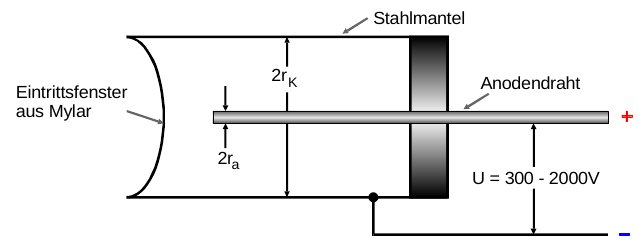
\includegraphics[width=0.8\textwidth]{pics/zaehlrohr.jpg}
\caption{Geiger-Müller-Zählrohr im Querschnitt$^{[1]}$}
\end{figure}
Im Zylinder selbst herrscht ein Unterdruck und er ist mit einem dünnen Argon-Alkohol-Gasgemisch gefüllt. Legt man nur eine Spannung zwischen Draht und Gehäuse an, so entsteht ein radialsymmetrisches elektrisches Feld mit der Feldstärke
\begin{align}
E(r)= \frac{U}{r\cdot \ln (r_k / r_a)}
\label{eq_efeld}
\end{align}
durch welches geladene Teilchen, die durch Ionisationsvorgänge im Zählrohr entstehen, zu den leitenden Flächen beschleunigt werden. Die ionisierten Atomrümpfe rekombinieren dort mit überschüssigen Elektronen aus der Kathode, während die Elektronen in der Anode abgeleitet und über einen Verstärker als Stromimpuls registriert werden.\\

Die Alkohol- und Edelgasatome werden durch die einfallende Strahlung ionisiert, die wahlweise $\alpha$-, $\beta$-, oder $\gamma$-Strahlung sein kann. Auf Grund ihrer kurzen Reichweite bzw. geringer Wechselwirkung eignen sich $\alpha \text{ und } \gamma$-Strahlen nicht so gut.

\subsection{Die Spannungsbereiche}
\label{sec_spannungsbereiche}
Je nachdem, wie hoch die an das Zählrohr angelegte Spannung ist, verhält sich das Zählrohr anders.

\begin{figure}[h]
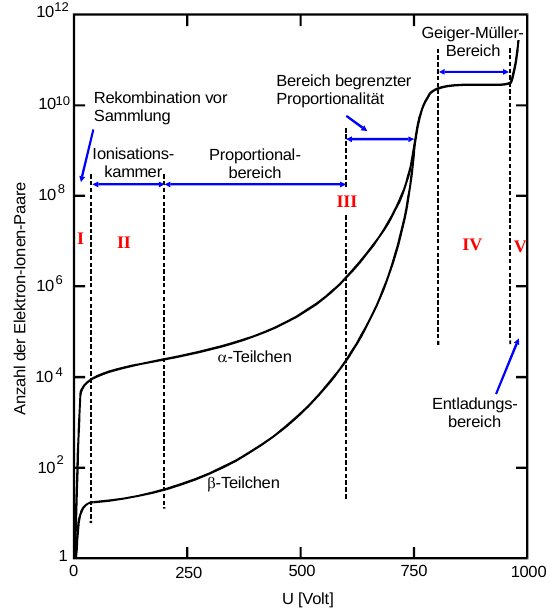
\includegraphics[width=0.6\textwidth]{pics/charak.jpg}
\caption{Charakteristik eines Zählrohrs für $\alpha$- und $\beta$-Strahlung$^{[1]}$}
\end{figure}

Ist die Spannung nur sehr gering, so rekombinieren die erzeugten Ionen mit den Elektronen, bevor sie Anode bzw. Kathode erreichen konnten. Es werden folglich nicht alle Ionisationsvorgänge registriert.

Erhöht man die Spannung weiter, werden schließlich quasi alle ionisierten Teilchen eingefangen. Der kontinuierlich zwischen Anode und Kathode fließende Ionisationsstrom ist dann proportional zur Energie und zur Intensität der einfallenden Strahlung. Unter diesen Bedingungen, stellt das Gerät eine Vorstufe zum Zählrohr dar und wird als Ionisationskammer bezeichnet. Sie eignet sich zwar nur bei hohen Strahlungsintensitäten, ermöglicht dort jedoch eine Messung der Strahlungsintensität, da der fließende Strom proportional mit ihr wächst.

Anschließend folgt ein Bereich, indem ionisierte Teilchen durch die Spannung so stark beschleunigt werden, dass sie ihrerseits andere Teilchen ionisieren können. Es entstehen sogenannte Townsend-Lawinen, deren Gesamtladung proportional zur Teilchenenergie ist, die die Strahlung abgegeben hat. Dadurch ist in diesem Bereich neben der Intensitätsmessung auch noch eine Energiemessung möglich. Man bezeichnet den Detektor in diesem Bereich daher auch als Proportionalitätszählrohr.

Das eigentliche Geiger-Müller-Zählrohr arbeitet im sog. Auslösebereich. Dort entstehen in der primären Elektronenlawine UV-Photonen infolge der Anregung von Argon-Atomen durch Elektronenstöße. Da die Photonen ladungsneutral sind, breiten sie sich auch senkrecht zum elektrischen Feld aus und erzeugen weitere Elektronenlawinen im gesamten Zählrohr. Die dann detektierte Ladung hängt nicht mehr von der Primärionisation, sondern nur noch von der Betriebsspannung und dem Zählrohrvolumen ab. Die freigewordene Ladung ist nun so groß, dass sie leicht nachgewiesen werden kann, es ist nun jedoch nur noch eine Intensitätsmessung möglich.

Erhöht man die Spannung weiter, so erzeugt jede Ionistation Kaskaden von Entladungen, durch die das Zählrohr nach kurzer Zeit zerstört wird.

\subsection{Tot- und Erholungszeit}
\label{sec_totzeit}
Bei der Ionistation werden nicht nur Elektronen, sondern auch erheblich schwerere positiv geladene Ionen erzeugt. Diese werden wegen ihrer hohen Masse nur langsam zur Kathode beschleunigt und verbleiben solange im Zählrohr, dass ihre positive Ladung die Feldstärke im Zählrohr soweit herabsetzt, dass für eine kurze Zeit keine eintreffenden Teilchen registiert werden können. Dies nennt man die Totzeit T des Zählrohrs.\\
Die Totzeit kann errechnet werden, indem man mit zwei Strahlungsquellen arbeitet. Zunächst plaziert man Quelle 1 vor dem Zählrohr und misst über eine bestimmte Dauer die entstehenden Impulse ($N_1$). Anschließend wird Quelle 2 zur Messung hinzugenommen und die durch beide Quellen entstehenden Impulse ($N_{1,2}$) simultan gemessen. Zu guter letzt entfernt man Quelle 1 und misst die Impulse von Quelle 2 alleine ($N_2$).\\
Setzt man die gemessenen Werte nun in folgende Formel ein:
\begin{align}
T\approx \frac{N_1+ N_2 - N_{1,2}}{2\cdot N_1 N_2},
\label{eq_totzeit}
\end{align}
so lässt sich die Totzeit den Zählrohrs näherungsweise bestimmen.

Während die Ionenwolke zum Mantel hin abwandert, steigt die Feldstärke wieder an und das Zählrohr kann weitere Teilchen registrieren. Solange das Feld jedoch noch nicht vollständig wiederhergestellt ist, haben folgende Primärimpulse eine geringere Intensität. Dieser Zeitraum $T_E$ wird daher Erholungszeit genannt.
\begin{figure}[htbp]
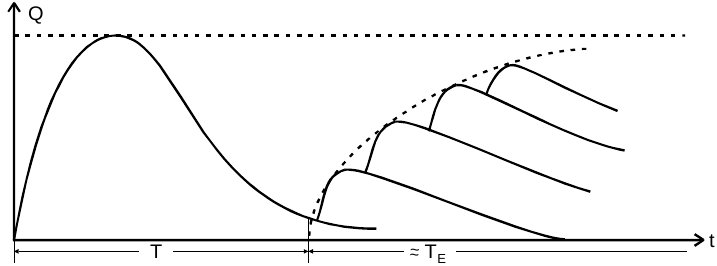
\includegraphics[width=0.8\textwidth]{pics/erholungszeit.jpg}
\caption{Tot- und Erholungszeit eines Geiger-Müller-Zählrohrs in einem Oszilloskop$^{[1]}$}
\label{pic_totzeit}
\end{figure}

\subsection{Nachentladungen}
Auch die auf die Mantelfläche treffenden Ionen können ihrerseits Hüllenelektronen ausschlagen, die weitere echoartige Kaskaden anregen. Diese sind höchst unerwünscht, da sie die Messung verfälschen und werden als Nachentladungen bezeichnet. Um sie zu minimieren wird dem Gas ein Alkoholanteil hinzugefügt, da die ionisierten Argonatome mit ihrer Energie wiederum die Alkoholatome ionisieren, welche keine Nachentladungen auslösen, sondern mit der Energie zu Schwingungen angeregt werden.

\subsection{Charakteristik}
Trägt man für ein Geiger-Müller-Zählrohr die registrierte Teilchenzahl N bei konstanter Strahlungsintensität gegen die angelegte Spannung U auf, so erhält man seine sogenannte Charakteristik.
Interessant ist insbesondere der Auslösebereich, der ein Plateau ausbildet. Bei einem idealen Zählrohr ist die Plateausteigung Null, jedoch wird immer eine geringe Steigung messbar sein, da Nachentladungen nie völlig ausgeschlossen werden können.
\begin{figure}[htbp]
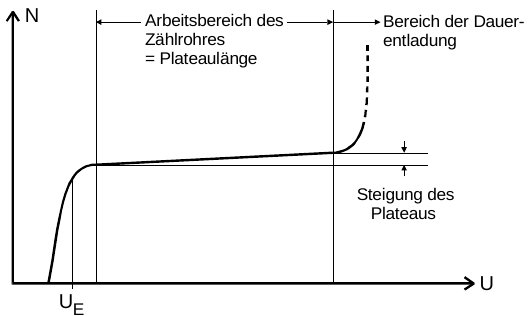
\includegraphics[width=0.8\textwidth]{pics/plateau.jpg}
\caption{Plateau des Auslösebereichs$^{[1]}$}
\end{figure}


\section{Durchführung}
Zunächst soll eine Charakteristik des Zählrohrs erstellt werden. Betrachtet wird hierzu eine $\beta$-Strahlungsquelle, die in einem
Abstand aufgebaut wird, so dass nicht mehr als 100 Impulse pro Sekunde gemessen werden. Auf diese Weise verliert die Totzeit an Bedeutung.
Zu verschiedenen Betriebsspannungen werden die Ionisationsvorgänge gemessen und ihre Anzahl gegen die Spannung in einem Diagramm
aufgetragen.

Die Totzeit kann ebenfalls mit Hilfe eines Oszilloskopes abgeschätzt werden. Man lässt dazu eine relativ hohe Strahlungsintensität in das Zählrohr fallen und betrachtet, wann der nächste Impuls frühestens gemessen werden kann.
Nachentladungen können sichtbar gemacht werden, indem man die Probe soweit entfernt, dass nur wenig Strahlung einfällt und dann die
Spannung des Zählrohrs auf ca 700V gestellt wird. Es werden nun Nachentladungen im Oszilloskop sichtbar, die qualitativ beschrieben
werden können. Hieraus lässt sich grob die Totzeit ermitteln
\begin{align}
\bar{I}:= \frac{1}{\tau} \int_0^\tau \frac{U(t)}{R}dt. \hspace{1cm} (\tau >> T)
\end{align}
Aus I lässt sich bei bekannter Impulsrate, die pro eindringendes Teilchen vom Zählrohr freigesetzte Ladungsmenge berechnen. Gemäß der Definition des Stromes als die pro Zeitintervall $\Delta t$ transportierte Ladungsmenge $\Delta Q$ gilt:
\begin{align}
\bar{I} = \frac{\Delta Q}{\Delta t} Z
\label{eq_ladung}
\end{align}
wenn Z Teilchen in der Zeit $\Delta t$ registriert wurden.
$\Delta Q$ hängt von der Zählrohrspannung U ab. Es ist daher zweckmäßig, $\Delta Q$ in Abhängigkeit von U zu untersuchen.


\section{Auswertung}
\subsection{Fehlerrechnung}
Da über ein großes Zeitintervall die Messungen gemacht werden, ist es hilfreich eine auf eine Sekunde genormte Zählung $Z$ einzuführen

\begin{equation}
 Z = \frac{N}{t}.
\end{equation}
Da gemessene Raten $N$ poissonverteilt sind, ergibt sich der absolute Fehler $\Delta Z$ zu

\begin{equation}
 \Delta Z = \frac{\sqrt{N}}{t}.
\end{equation}
Fehler von Größen, die von mehreren fehlerbehafteten Größen abhängig sind errechnen sich aus der Gaußschen Fehlerfortpflanzung

\begin{formel}[H]
\begin{equation}
\Delta G = \sqrt{\sum_{i=1}^{N}\left( \frac{\partial G}{\partial x_i}\cdot \Delta x_i\right)^2}.
\label{eq_gauss}
\end{equation}
\caption*{\small{$x_i$ = Variable, $\Delta x_i$ = Fehler der Variable}}
\end{formel}

\subsection{Charakteristik des Geiger-Müller-Zählrohrs}
Die benutzte Strahlungsquelle ist das Thallium-Isotop $^{204}$Tl und wird für das Erstellen der Zählrohrstatisktik verwandt. Bei
verschiedenen Spannungen $U$ ergeben sich $N$ gemessene Impulse, sowie ein Zählrohrstrom $I$. In Tabelle \ref{tab_charakteristik} sind diese
Größen aufgeführt.

\begin{table}[H]
 \begin{tabular}{c|c|c|c|c}
 $U$ in V & $N$ in 1/s & $Z$ in 1/s & $\Delta Z$ in 1/s & $I$ in $\mu$A \\
 \hline
  332&	114 &0,57&	0,053&	0,000 \\
334&	5803 &29,02&	0,381&	0,080\\
335&	14425&	72,13&	0,601&	0,080\\
340&	14691&	73,46&	0,606&	0,080\\
350&	14543&	72,72&	0,603&	0,090\\
400&	14667&	73,34&	0,606&	0,100\\
450&	14834&	74,17&	0,609&	0,130\\
500&	15030&	75,15&	0,613&	0,205\\
550&	14973&	74,87&	0,612&	0,250\\
600&	15126&	75,63&	0,615&	0,290\\
650&	15459&	77,30&	0,622&	0,320\\
670&	15790&	78,95&	0,628&	0,325\\
700&	16429&	82,15&	0,641&	0,400\\
710&	17049&	85,25&	0,653 &	0,400\\
 \end{tabular}
\caption{Impulse und Strom zu Spannungen bei $t$ = 200s}
\label{tab_charakteristik}
 \end{table}

Bei Betrachtung der Werte, kann man ein Sättigungsverhalten der Impulse bei dem Spannungsbereich von 335 V und 670 V feststellen. In
Abbildung \ref{pic_plateau} wird die Gerade \eqref{eq_charak} mittels GNUplot gefittet, sodass die nicht verhinderbare Steigung des Plateaus ermittelt
werden kann.

\begin{align}
 N = a\cdot U + b
 \label{eq_charak}
\end{align}


\begin{figure}[H]
 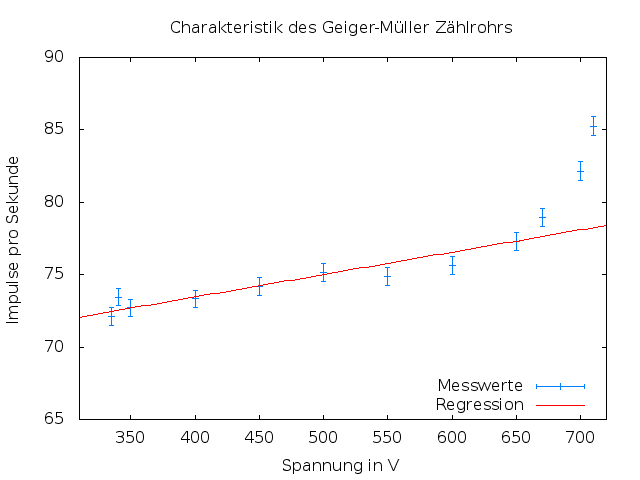
\includegraphics[width=0.8\textwidth]{pics/charakteristik.png}
 \caption{Charakteristik des Geiger-Müller-Zählrohrs}
 \label{pic_plateau}
\end{figure}
Besagte Plateausteigung beträgt somit 
\begin{align}
a = (2,09 \pm 0,26)\%/100\text{V} \intertext{mit Y-Achsenabschnitt} b = (67,28 \pm 0,96) \text{V}.
\end{align}


\subsection{Bestimmung der Totzeit mittels Oszilloskop}
Auf einem Oszilloskop werden die gemessenen Impulse als Wellenberge entsprechend Abbildung \ref{pic_totzeit} dargestellt. Ab einer
Spannung von etwa 350 V erscheinen die Nachentladungen auf dem Schirm. Bei einer Spannung von $U$ = 700 V und einer bekannten
Ablenkspannung von etwa 50 $\mu$s/cm wird der Abstand der Peaks vom einfallenden Teilchen, sowie der schnellsten Nachentladung zu
$b$ = 2,5 cm abgeschätzt, was zu einer groben Näherung der Totzeit mit $T$ = 125 $\mu$s führt.

\subsection{Bestimmung der Totzeit mittels Zwei-Quellen-Methode}
Wie in Abschnitt \ref{sec_totzeit} beschrieben, wird die 2-Quellen-Methode bei einer Spannung $U$ = 700 V durchgeführt.

\begin{table}[H]
 \begin{tabular}{c|c|c|c}
Probe & $N$ in 1/s & $Z$ in 1/s & $\Delta Z$ in 1/s \\
\hline
$N_1$	& 12709 & 63,55 & 0,564\\
$N_2$ & 54976 & 274,88 & 1,172\\
$N_{1,2}$ & 65606 & 328,03 & 1,281
  
 \end{tabular}
\caption{Messungen zur Zwei-Quellen-Methode bei $t$ = 200s}
\label{tab_2quellen}
\end{table}

Mit den Werten aus Tabelle \ref{tab_2quellen} lässt sich mittels Gleichung \eqref{eq_totzeit} die Totzeit errechnen. Der Fehler ergibt
sich aus Gleichung \eqref{eq_gauss}.

\begin{align}
 T = (297,6 \pm 50,7) \mu s
\end{align}

\subsection{Messung freigesetzter Ladungsmenge}
Ein ins Geiger-Müller-Zählrohr eintretende Teilchen sorgt bei hohen Spannunge wie in \ref{sec_spannungsbereiche} beschrieben, für sehr
viele Ladungen, die auf den Anodendraht treffen. Das hat einen Stromfluss zufolge, welcher in Tabelle \ref{tab_charakteristik}
aufgeführt ist. Die Anzahl an Ladungsträgern errechnet sich aus Gleichung \eqref{eq_ladung} und ist in Tabelle \ref{tab_ladungsmenge}
in Abhängigkeit der Stromstärke gezeigt. Via GNUplot wird die Gleichung
\begin{align}
 \frac{Q}{e} = c\cdot U + d
\end{align}
gefittet. In Abbildung \ref{pic_ladung} sind die Ergebnisse zu sehen.

\begin{table}[H]
\begin{tabular}{c|c|c|c}
$U$ in V & $Z$ in 1/s & $I$ in $\mu$A & $Q$ in 10$^{10}\,e$\\
\hline
332	&0,57&	0,000&	0,000\\
334&	29,02&	0,080&	1,721\\
335&	72,13&	0,080&	0,692\\
340&	73,46&	0,080&	0,680\\
350&	72,72&	0,090&	0,773\\
400&	73,34&	0,100&	0,851\\
450&	74,17&	0,130&	1,094\\
500&	75,15&	0,205&	1,703\\
550&	74,87&	0,250&	2,084\\
600&	75,63&	0,290&	2,394\\
650&	77,30&	0,320&	2,584\\
670&	78,95&	0,325&	2,570\\
700&	82,15&	0,400&	3,040\\
710&	85,25&	0,400&	2,929 \\

\end{tabular}
\caption{freigesetzte Ladung $Q$ bei verschiedenen Spannungen}
\label{tab_ladungsmenge}
\end{table}

\begin{figure}[H]
 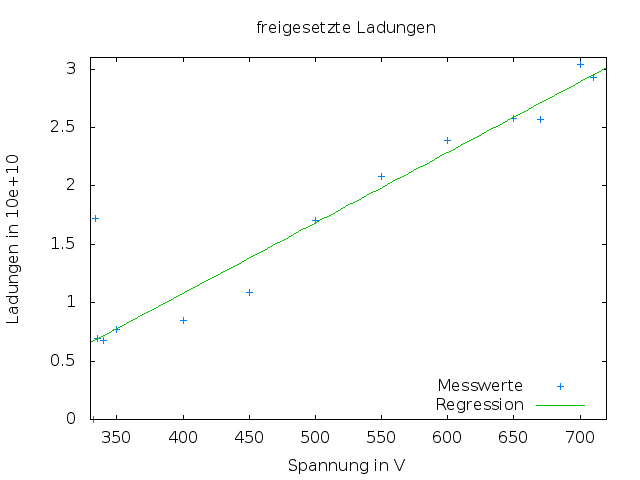
\includegraphics[width=0.8\textwidth]{pics/ladungen.png}
 \caption{durch einfallende Teilchen freigesetzte Ladung bei verschiedenen Spannungen}
 \label{pic_ladung}
\end{figure}
Der Regressionsfaktor wird mit 
\begin{align}
c = (6,03 \pm 0,70)\cdot 10^{9} \, \text{Ladungen/100V} \intertext{mit Y-Achsenabschnitt} d = (-1,33 \pm 0,36) \cdot 10^{12} \, \text{Ladungen}.
\end{align}

\section{Diskussion}
Das Plateau in der Charakteristik des Geiger-Müller-Zählrohrs ist mit einer Steigung von etwa 2\%/100V durchaus gut feststellbar
und entspricht den Erwartungen. Zur besseren Abstimmung der Grenzen sind an den Randwerten mehrere Messungen durchgeführt worden.

Die Messungen zur Totzeit beider Methoden sind gut miteinander vergleichbar. Der Wert des Oszilloskops beläuft sich auf
$1,25 \cdot 10^{-4}$s. Die Ermittlung über die Zwei-Quellen-Methode ergibt einen vergleichbaren mit $2,98 \cdot 10^{-4}$s. Also ist
davon auszugehen, dass das Ergebnis dem realen Wert nahe kommt.

Im Plateaubereich scheint für die freigesetzten Ladungen ein linearer Zusammenhang zur Spannung zu bestehen. Da nach Gleichung \eqref{eq_efeld}
das elektrische Feld proportional zur Spannung ist, kann auch dieses Phänomen erklärt werden.

\parskip 50pt
\Large{Literatur}\\\\
\large{[1] Versuchsanleitung - Das Geiger-Müller-Zählrohr}\\\\
% ========================================
% Literaturverzeichnis
% ========================================

%\bibliographystyle{plainnat} % Bibliographie-Style auswählen
%\bibliography{BIBDATEI} % Literaturverzeichnis

% ========================================
% Das Dokument endent
% ========================================

\end{document}